\documentclass{scrartcl}
\usepackage{graphicx} % Required for inserting images
% \usepackage{url}
\usepackage{xurl}
\usepackage{authblk}
\usepackage[hidelinks]{hyperref}
\usepackage[nomarkers]{endfloat}
\usepackage[toc,page]{appendix}
\usepackage[
    backend=biber,
    style=numeric
]{biblatex}
\addbibresource{main.bib}

\title{To See Oursels as Ithers See Us}
\subtitle{Updating the Melville Monument, Edinburgh 2016 - 2025}
\author[1]{Matthew Hamilton}
\author[2]{Agnes Michalczyk}
\author[3]{Marianna Vanessa Buoni Pineda}
\affil[1]{Università di Bologna}
\affil[2]{University of}
\affil[3]{University of}
\date{}

\begin{document}

\maketitle

\begin{abstract}
Since the Acts of Union in 1707, Scotland’s relationship with England has been at times strained. 
Scotland as a nation has historically viewed itself as ‘under English rule’, rather than as an equal participant in British colonialism and empire. 
For this reason, Scotland has evaded a reckoning with its involvement in the slave trade. 
During the Black Lives Matter demonstrations in 2020, there was a growing call for reflection into Scotland’s profiting from slavery and its contribution to now heritage architecture. 
One such architectural piece was the Melville Monument in St. Andrew's Square, Edinburgh. 
This article explores the debate and happenings around the installation of a new plaque on the monument, beginning with the original petition up until the present day.
Outlined are the main actors in the debate, their motivations, the timeline of the plaques installation and reflection in the wider context of similar cases in Edinburgh and the wider Scottish heritage sector.
\end{abstract}

\section{TODO}:

\begin{itemize}
    \item Rewrite Abstract
    \item Fill in bullet points of:
    \begin{itemize}
        \item Introduction (Agnes)
        \item Existing Work
        \item Case Study
    \end{itemize}
    \item Get OS map of St Andrew's Square (Matthew)
    \item Organise Links (Matthew)
    \item Proofread (everyone)
    \item Author Data
    \begin{itemize}
        \item Add university affiliations (everyone)
    \end{itemize}
    \item Outline slides
    \begin{itemize}
        \item Themes
        \item Main points
        \item gather assets
    \end{itemize}
    \item Upload introduction or Footnotes and the
\end{itemize}

\section{ Slides}

List of slides, there theme and main points to hit

\begin{itemize}
    \item Introduction (Agnes)
    \begin{itemize}
        \item Slide1: (Intro) Introduce the presentation    
        \item Slide2: (Historical Context) give context on the nation-state    
        \begin{itemize}
            \item cast light on European contexts 
            \item shaped by different colonial and imperial histories and racial formations
        \end{itemize}        
        \item Slide3: (History of Heritage Policy) expose discussion and evolution of heritage policies        
        \begin{itemize}
            \item within the context of antiracist and decolonial movemens
        \end{itemize}
    \end{itemize}
    \item Lit review (Agnes)
    \begin{itemize}
        \item Slide4: (Theme) critical review of relevant literature
    \end{itemize}
    \begin{itemize}
        \item Slide5: (Theme) critical review of relevant literature
    \end{itemize}
    \begin{itemize}
        \item Slide6: (Theme) critical review of relevant literature
    \end{itemize}
    \item Case Overview: (Matthew)
    \begin{itemize}
        \item Slide7: (Introduce Melville Debate) public debate of melville monument 
        \begin{itemize}
            \item contestations around a monument.
            \item history of the monument
        \end{itemize}
    \end{itemize}
    \begin{itemize}
        \item Slide8: (Henry Dundas)
        \begin{itemize}
            \item who was henry dudas
        \end{itemize}
    \end{itemize}
    \item Actors (Matthew)
    \begin{itemize}
        \item Slide9: (Main players)
        \begin{itemize}
            \item For Plaque
            \item Against
            \item Academic commentators
        \end{itemize}
        \item Slide10: (Discourse) analyse their discourses. 
        \begin{itemize}
            \item In media
            \item in publications
        \end{itemize}
    \end{itemize}
    \item Debate (Matthew)
    \begin{itemize}
        \item Slide11: (``Trouble''): make visible the \textit{trouble} around these heritage monuments
        \begin{itemize}
            \item defacing
            \item demonstrations
            \item theft
        \end{itemize}
    \end{itemize}
    \item Response (Matthew / Marianna)
    \begin{itemize}
        \item Slide12: explore the role of a set of actors:
        \begin{itemize}
            \item 
        \end{itemize}
    \end{itemize}
    \begin{itemize}
        \item Slide13:
    \end{itemize}
    \begin{itemize}
        \item Slide14:
    \end{itemize}
    \item Aftermath (Marianna)
    \begin{itemize}
        \item Slide15:
    \end{itemize}
    \begin{itemize}
        \item Slide16:
\end{itemize}
\item Conclusion (Marianna)
    \begin{itemize}
        \item Slide17:
    \end{itemize}
    \begin{itemize}
        \item Slide18:
    \end{itemize}
    \begin{itemize}
        \item Slide19:
    \end{itemize}
    \begin{itemize}
        \item Slide20:
    \end{itemize}
\end{itemize}

\section{Bulleted Points}

The main points the presentation / article needs to hit:

\begin{itemize}    
    \item give context on the nation-state     
    \item cast light on European contexts (shaped by different colonial and imperial histories and racial formations)
    \item expose discussion and evolution of heritage policies within the context of antiracist and decolonial movements
    \item critical review of relevant literature.
    \item focus on a public debate that has taken place recently: raised by contestations around a monument. 
    \item identify the different actors involved in this debate \ref{actors}
    \item analyse their discourses. 
    \item analyse alternative heritage practices such as (artistic intervention, walking tour etc.).
    \item make visible the \textit{trouble} around these heritage monuments
    \item explore the role of a set of actors:
    \begin{itemize}
        \item that contribute to produce knowledge on the legacies of colonialism in Europe
        \item  and create counter-hegemonic narratives and memories.
        \item in relation with institutional cultural institutions        
    \end{itemize}
\end{itemize}

\section{Introduction}

\begin{itemize}
    \item context on the nation-state 
    \begin{itemize}
        \item For context of construction of Melville's monument see \cite{godard_2018}
    \end{itemize}
    \item cast light on European contexts (shaped by different colonial and imperial histories and racial formations)
\end{itemize}


The enduring legacies of the transatlantic slave trade continue to provoke critical re-evaluation of national narratives and heritage policies across Europe. To understand the complexities of these legacies, we must first acknowledge the nation-state not as an immutable entity, but as a historically contingent construct. As Benedict Anderson famously argued in Imagined Communities (2006), the nation is an “imagined political community”—a collective identity forged through shared narratives, symbols, and experiences.

This construction, however, is not neutral; it often serves to consolidate power, privilege certain histories, and obscure uncomfortable truths. In the context of European colonialism and the slave trade, the nation-state became a vehicle for legitimizing and perpetuating systems of exploitation. Consequently, the narratives that underpin national identity are frequently intertwined with the histories of empire and racialized power, demanding a critical lens that acknowledges the selective nature of historical memory and the persistent challenge of decolonizing national consciousness.  
The ongoing interrogation of historical legacies stemming from the transatlantic slave trade has prompted a critical re-evaluation of national narratives and heritage policies across Europe. 
This article contributes to this discourse by examining the intertwined histories of Scotland and the Caribbean, focusing on the enduring impact of slavery and its subsequent memorialization within the Scottish metropolis. 
The nation-state, as a construct, is not a monolithic entity but rather a product of specific historical forces, including colonialism and imperialism \cite{godard_2018}.
Understanding the nation-state requires acknowledging its role in shaping and being shaped by these forces, particularly in the context of European expansion and exploitation. 
As Anderson (2006) argues, national identity is an "imagined community," constructed through shared narratives and symbols, often obscuring or sanitizing uncomfortable historical realities.1
This article extends beyond a purely national framework by casting light on the diverse European contexts that have shaped, and continue to be shaped by, different colonial and imperial histories and racial formations.
Europe's engagement with the slave trade was not uniform; rather, it involved a complex web of actors, institutions, and ideologies that produced distinct racialized hierarchies and power structures (Goldberg, 2002) \cite{goldberg_2002}.
Consequently, the legacies of slavery manifest differently across European nations, necessitating a nuanced approach that considers the specific historical trajectories and cultural contexts of each region.
In Scotland, as demonstrated by the works of Alston \cite{alston_2021} and studies of the "Glasgow Sugar Aristocracy," the economic and social impact of slavery was profound, yet often obscured by narratives of Scottish exceptionalism.

Furthermore, the memorialization of this history, as exemplified by monuments like the Melville Monument \cite{godard_2018}, reveals how dominant narratives have been embedded within the urban landscape, reinforcing particular interpretations of the past.2 The increasing demands for apologies and reparations \cite{hartel_2024}, driven by anti-racist and decolonial movements, highlight the ongoing contestation of these narratives and the urgent need for a critical reassessment of heritage policies.3 This article aims to contribute to this reassessment by analysing the interplay between historical scholarship, memorialization, and contemporary debates on historical justice, ultimately revealing the dynamic evolution of heritage policies within the context of anti-racist and decolonial movements.

\section{Existing Work}

\begin{itemize}
    \item expose discussion and evolution of heritage policies within the context of antiracist and decolonial movemens
    \item critical review of relevant literature.
\end{itemize}

This review examines key works that contribute to a deeper understanding of the complex and often obscured legacies of the transatlantic slave trade in Scotland and Britain, and how these legacies are being re-evaluated within the context of anti-racist and decolonial movements: David Alston's "Slaves and Highlanders: Silenced Histories of Scotland and the Caribbean" \cite{alston_2021}, an analysis of the "Glasgow Sugar Aristocracy" \cite{mullen_2022} Lisa Ellen Hartel's "Legacies of the Slave Trade: An Analysis of Demands, Apologies and Reparations in Britain over the Last 25 Years" \cite{hartel_2024} , and Clarisse Godard Desmarest's "The Melville Monument and the Shaping of the Scottish Metropolis" (2018) \cite{godard_2018}.
Alston's "Slaves and Highlanders" provides a crucial corrective to the prevailing narratives that often minimize or overlook Scotland's role in the slave system. 
Alston reveals the extent to which wealth derived from enslaved labour permeated Scottish society by focusing on the disproportionate involvement of Highland Scots, particularly in the later stages of the slave trade.
By meticulously documenting the presence of Highlanders as plantation owners, managers, and merchants in the Caribbean he challenges the "silenced histories".
This work highlights the importance of regional specificity in understanding the impact of slavery, demonstrating how certain communities within Britain were deeply entangled in the system.
 Furthermore, moving beyond a purely economic analysis and laying groundwork for decolonial readings of Scottish history, Alston's commitment to amplifying the voices of the enslaved and free people of colour underscores the human cost of this historical relationship.
The study of the "Glasgow Sugar Aristocracy" is complementing Alston's regional focus and expands the analysis to encompass the broader economic impact of Caribbean slavery on British society.
It examines the role of West India merchants and planters in shaping the economic landscape of Glasgow, highlighting the flow of capital from the colonies to the metropole.
This work emphasizes the interconnectedness of colonial and metropolitan economies, demonstrating how profits from enslaved labour fuelled industrial and agricultural development in Britain.
Focusing on the "repatriated slavery fortunes," it provides insights into the tangible ways in which wealth derived from slavery was integrated into British society, thereby informing contemporary discussions on reparative justice.
Godard Desmarest's analysis of the Melville Monument adds a crucial dimension by illuminating the ways in which the wealth and power derived from colonial exploitation were publicly memorialized and integrated into the urban fabric of the Scottish metropolis.
The monument, dedicated to Henry Dundas, a key figure in delaying the abolition of the slave trade, serves as a powerful symbol of the elite's investment in and endorsement of the colonial system underscoring how public architecture and monuments were used to solidify social hierarchies and reinforce the legitimacy of colonial power.
Crucially, in the context of anti-racist and decolonial movements, Desmarest’s work highlights how such monuments have become sites of contestation and re-evaluation, forcing a re-examination of heritage policies and the narratives they perpetuate.

Hartel's contemporary analysis, "Legacies of the Slave Trade," brings the discussion into the present day, examining the evolving discourse surrounding Britain's historical responsibility.
Her work reveals the significant increase in demands for apologies and reparations over the past 25 years, reflecting a growing awareness of the enduring legacies of slavery.
Hartel's analysis of the reparations debate highlights the complexities and challenges associated with addressing historical injustices, including the different forms reparations might take and the political and social obstacles to their implementation.
This work underscores the ongoing struggle to reconcile with the past and the need for a more nuanced understanding of historical accountability, directly impacting and being impacted by, the evolution of heritage policies within anti-racist movements.
Collectively, these works contribute to a more comprehensive understanding of the multifaceted legacies of slavery in Scotland and Britain.
Alston's work emphasizes the regional specificity and human cost of the system, while the study of the "Glasgow Sugar Aristocracy" illuminates the economic impact on the metropole.
Godard Desmarest demonstrates how these economic and political powers were visually expressed and preserved in the metropolitan landscape and how that landscape is being contested.
Hartel's contemporary analysis demonstrates the ongoing struggle to address historical injustices and the enduring relevance of the reparations debate, and how that struggle is shaping and being shaped by the evolution of heritage policies within anti-racist and decolonial movements.
By combining historical research with contemporary analysis of both written and built history, these works provide a critical foundation for understanding the complex and enduring legacies of slavery in British society and the ongoing efforts to decolonize its historical narratives.

\section{Case Study: Melville's Monument}

\begin{itemize}
    \item focus on a public debate that has taken place recently: raised by contestations around a monument. 
    \item identify the different actors involved in this debate \ref{actors}
    \item analyse their discourses. 
\end{itemize}

\subsection{Timeline}

\begin{itemize}
    \item 1938 Eric Williams writes \url{https://www.theguardian.com/world/2022/jan/23/eighty-years-late-groundbreaking-work-on-slave-economy-is-finally-published-in-uk}
    \item 1975: Critique of Dundas from David Brion Davis \cite{davis_1975}
    \item May 2016: \textit{idea of a plaque on the statue first raised its head in 2016, when Adam Ramsay, the editor of OpenDemocracy, started a petition which was handed into the council.}\cite{anderson_2021} \url{https://www.edinburgh.gov.uk/directory-record/1110080/a-plaque-for-the-melville-monument}
    \begin{itemize}
        \item At some point between the time around the petition and 12th Aug, Adam Ramsay installs his own plaque which is taken down by the council.
    \end{itemize}
    \item 5 October 2017: Urquhart Media \url{https://www.youtube.com/watch?v=LL3IKRIPIUc}
    \item 12 Aug 2018: Channel 4 news broadcasts piece on the plaque \cite{c4n_2018} Confirming Geoff Palmer, Adam Ramsay, Bobby Dundas, and Michael Fry as part of the ``plaque committee'' \ref{fig:plaque-committee}. In the course of the news item: ``Edinburgh [Council] Wants new wording by September [2018]''
    \item  June 2020: Inciting action: \textit{In June 2020, during a Black Lives Matter demonstration in the city, the monument was vandalised.}\cite{anderson_2021}  in particular the defacing of Melville's monument and the statue of his son Robert Dundas \cite{hay_2020_3} just a couple of days after Geoff Palmer calls for the plaque to be installed \cite{hay_2020_1} and the day after installation of the plaque would be expedited \cite{hoffman_2020, daily_2020} 
    \begin{itemize}
        \item initial debate summer of 2020 debate\cite{mccarthy_2022}
        \item 7 June 2020: (Side Note) Statue of Edward Colston toppled in Bristol, which was a factor in galvanising action on the Melville Monument 
        \item 7 June 2020: Geoff Palmer speaks at Black Lives Matter demonstrations and talks prominently of Dundas. Within he following days, the monuments to Dundas and his son would be defaced \cite{hay_2020_3} 

    \end{itemize}
    \begin{itemize}
        \item September 2020: (Side Note) University of Edinburgh rename David Hume Tower \url{https://www.ed.ac.uk/news/students/2020/equality-diversity-and-inclusion-an-update}/ [consec: \url{https://www.bbc.co.uk/news/uk-scotland-edinburgh-east-fife-54138247}]
    \end{itemize}
    \item March 2021, Edinburgh City Council  installs a new plaque  \cite{mccarthy_2022}\cite{anderson_2021}
    \item March 2023: call for plaque removal by Melville Monument Committee (descendants of Henry Dundas)  \cite{bbc_2023}
    \item September 2023. plaque `removed' or `stolen' 17 October 2023  by Melville Monument Committee \cite{bbc_2024}
    \item March 2024: New plaque: same wording \cite{bbc_2024} \url{https://www.edinburgh.gov.uk/news/article/13940/replacement-plaque-installed-at-the-melville-monument}
\end{itemize}

\begin{quotation}
    Can one wonder that Dundas, 
            opposing Wilberforce’s motion of 1792, 
                    on the ground that abolition should be: 
                    “gradual, that is, that time should be allowed to the planters to purchase sufficient supplies so that they should be well stocked when abolition took place,'' ?
    Can one wonder that Dundas, 
                                            %so determined an enemy of abolition, 
    moved the immediate abolition of the foreign slave trade, 
     which, 
                                             %according to him, 
    amounted in 1791 to 34,000 out of 74,000 imported?
\end{quotation}
\cite{williams_1938}

but williams also says

\begin{quotation}
    Even Dundas, who was in reality the friend of the West Indians [plantation owners], admitted that the desire to increase the cultivation of the West Indian Islands was no good cause for continuing so unjust a traffic as the slave trade. Page 20
\end{quotation} 
see \cite{williams_1938}[Page 27-28]

\subsubsection{A Note on Dates}

I have found it fascinating how sloppy the citing of key dates is when trying to assemble a timeline. This speaks more to the the methodology side side, but even after just a couple of years, the certainty around  key dates becomes tarnished, in particular the date the plaque was installed, the date it was removed and when it was reinstalled.

see here for how quickly the facts get blurred \url{http://melbourneblogger.blogspot.com/2025/01/melville-monument-edinburgh-pull-down.html}

\subsection{The Actors}\label{actors}

\begin{itemize}
    \item Edinburgh Slavery and Colonialism Legacy Review Group (ESCLRG): Group charged of reviewing heritage architecture in Edinburgh and their naming in order document links to colonial slavery and suggest action to address it. Criticised by academics such as Rowland. McCarthy and Devine for lack of representation of historians in the group.
    \begin{itemize}
        \item Chair: Professor \textbf{Sir Geoff Palmer} and Jamaica’s first honorary consul in Scotland. Member of original  ``plaque committee'' \cite{hay_2020_2}. Spoke at BLM demonstration \url{https://theedinburghreporter.co.uk/2020/06/video-sir-geoffrey-palmer-at-black-lives-matter-in-edinburgh/} . Author of ``Mr White and the Ravens'' and ``The Enlightenment - Citizens of Britishness'', and is Honorary President of the Edinburgh and Lothian Regional Equality Council.
    \item Edinburgh City council leader: \textbf{Adam McVey}
    \end{itemize}
    \item human rights activist \textbf{Adam Ramsay}
    \item Caribbean historian\textbf{ Eric Williams} (described Dundas as a determined ‘enemy of abolition’) \cite{mullen_2021}
    \item  Melville Monument Committee
    \begin{itemize}
        \item \textbf{Bobby Dundas}: 10th Viscount Melville
        \begin{itemize}
            \item and sister
        \end{itemize}
    \end{itemize}
    \item \textbf{Benjamin Carey}: Dundas descendant who called for the plaque
    \item \textbf{Professor Guy Rowlands}:  Professor of History at St Andrews \textit{has also judged the plaque ‘deeply misleading’ and ‘egregiously unfair’}  \cite{mccarthy_2022, rowlands_2021}
    \item \textbf{Tom Devine}: Critical of Dundas \cite{devine_2015}, but critical also of the wording of the new plaque. Was in a public spat with Geoff Palmer.
    \item \textbf{Angela McCarthy}: New Zealand academic in the field of Scottish migrations. Like Devine, critical of Dundas but also of the ESCLRG report \cite{esclr_2022}
\item \textbf{Michael Fry}: Scottish Historian and Biographer of Dundas \cite{fry_1992}. Was asked to draft the wording of the new plaque \cite{mccarthy_2022}\footnote{Possibly from \url{https://www.thenational.scot/comment/18519171.real-truth-henry-dundas-whether-prolonged-slavery/}}
\item \textbf{Lisa Williams}: (Research Associate at the Royal Botanic Gardens Edinburgh and an Honorary Fellow in the School of History, Classics and Archaeology at the University of Edinburgh.)

\end{itemize}

\textit{Professor Sir Geoff Palmer, Jamaica’s first honorary consul in Scotland, and the human rights activist Adam Ramsay led a high-profile campaign to reword the plaque on Edinburgh’s Melville monument, upon which a statute of Henry Dundas is mounted}\cite{mullen_2022}

\subsubsection{Note on Social Class In the UK}

This is a little hand wavy, but I feel it is worth noting social classic as a vector of influence in the debate. Those in standing in defence of Dundas are typically from monied or higher class backgrounds. Bobby Dundas is obviously a descendant of Dundas (rather that we don't look too closely lest the source of wealth is brought into question). Michael Fry , not much in way of history, but attended University of Oxford. Enrolment at Oxford is massively skewed to higher classes / privately educated individuals, especially at the time Fry attended. Not a stretch to assume Fry has upper class leanings.    

Contrast with Geoff Palmer and Tom Devine. Devine is from a working class Scottish background. Geoff Palmer is Jamaican, mother was Windrush. It  is probable that the friction between Devine and palmer comes from their separate experience, in particular Devine who had not experienced a side of the UK that Palmer would have.

In the UK Class divides people sooner than race compared to many other nations. However, those from different racial background would likely disagree at how quickly ``class over race'' as a rule for order of precedence in societal divisions.  Palmer and Devine come from very different racial backgrounds, with Palmer experiencing a side of the UK that Devine has not. This  is particularly pertinent when Devine is declaring what is and what is not important with respect to the removal or renaming of places as it relates to Afro-Caribbean black history and slavery.

\subsection{The Debate}

\begin{itemize}
    \item public debate about Melville monument in Scotland
    \begin{itemize}
        \item it's origin
    \end{itemize}
    \begin{itemize}
        \item and about the monument
    \end{itemize}
    \item identify the different actors involved in this debate
    \begin{itemize}
        \item analyse their discourses
    \end{itemize}
\end{itemize}

The debate centres around Henry Dundas, 1st Viscount Melville and whether the changes he made for `gradual' implementation to legislation presented by William Wilberforce on the abolition.

\begin{quotation}
    He spoke during parliamentary debates on abolition of the British slave trade, including in 1792 when he proposed a motion for gradual delay when the House of Commons was set to reject William Wilberforce’s proposal for abolition. 
\end{quotation}
\cite{mullen_2021}

To over simplify, the debate rests on two sides:

\begin{enumerate}
    \item Henry Dundas knowingly delayed the cessation of the slave trade to the benefit of xx
    \begin{itemize}
        \item assumes that Dundas would gain from the delay.
    \end{itemize}
    \item Henry Dundas saved the legislation by adding the `gradual' clause to make it more palatable 
    \begin{itemize}
        \item assumes the legislation was guaranteed to fail without intervention
    \end{itemize}
\end{enumerate}

During the Black Lives Matter demonstration in Edinburgh in June 2020 the monuments to Dundas and his son were a focal point and targeted with graffiti (Image Needed). 

It is popularly reported that the debate began with these demonstration, but a petition was made and approved 4 years previous in 2016 by Adam Ramsay \cite{mullen_2021} for a new plaque outlining who Dundas was and the controversies of his actions. Wording of the plaque was assigned to a committee which included at least Michael Fry, a Dundas biographer and ``defender \textit{par excellence}'' \cite{mccarthy_2022}, but it languished for a number of years.

In response to the protests the Edinburgh City Council pushed for the new plaque to be finished with Sir Geoff Palmer advising. Professional historians were absent from the process of deciding the wording \cite{scotsman_2022}. NOTE: There is equally no coverage of who was approached to be part of the plaque committee or the ESCLRG and it is equally possible some historians were asked to participate, but none showed interest.

\subsubsection{Quotes}
\begin{quotation}{Sir Geoff Palmer in \cite{anderson_2021}}
    “I can assure you that some of the people who don’t want this plaque, with slavery on it, they would rather the statue would come down, because that’s the power of the plaque and the truth of the plaque.
\end{quotation}
\begin{quote}
    Bobby Dundas had previously criticised the inscription as being written by "non-historians at the height of the Black Lives Matter demonstrations in 2020".
\end{quote}\cite{bbc_2024} though the call for a plaque began in 2016, 4 years prior.

\subsubsection{Black Lives Matter Demonstrations, Edinburgh, June 2020}

Geoff palmer speaks at the demonstration of the Dundas statue and how he had been on the committee for 2 years. \url{https://www.youtube.com/watch?v=44Evo9iZtow}

\subsection{The Response}

This section should cover:

\begin{itemize}
    \item ``analyse alternative heritage practices''
    \begin{itemize}
        \item  (artistic intervention, walking tour etc.).
        \begin{itemize}
            \item \url{https://blackhistoryscotland.com} and \url{https://www.edinburghlive.co.uk/news/history/woman-behind-edinburghs-black-history-21738094}
        \end{itemize}
        \begin{itemize}
            \item Does graffiti count? \url{https://www.edinburghnews.scotsman.com/news/crime/these-pictures-show-the-second-melville-statue-in-edinburgh-defaced-following-black-lives-matter-protest-2879014}. Dundas is called out as a slaver, but he did not trade in slaves directly.
        \end{itemize}
    \end{itemize}
    \item make visible the \textit{trouble} around these heritage monuments
    \item explore the role of a set of actors
    \begin{itemize}
        \item that contribute to produce knowledge on the legacies of colonialism in Europe and create counter-hegemonic narratives and memories.
        \item in relation with institutional cultural institutions
        \begin{itemize}
            \item Note: \textit{the debacle influenced an investigation in Toronto, Canada, into the renaming there of Dundas Street} \cite{mccarthy_2022}
        \end{itemize}
    \end{itemize}
\end{itemize}

Calls for how to respond to the debate in 3 flavours

\begin{enumerate}
    \item Do Nothing \url{https://www.melvillemonument.com/statement/}
    \item Removal \url{https://www.scotsman.com/news/opinion/columnists/henry-dundass-statue-in-edinburgh-should-be-torn-down-over-slave-trade-links-martyn-mclaughlin-2879038} and \url{https://www.change.org/p/remove-the-statue-of-henry-dundas-and-rename-the-streets-named-after-him-in-edinburgh?recruiter=false&utm_source=share_petition&utm_medium=twitter&utm_campaign=psf_combo_share_initial&utm_term=psf_combo_share_initial&recruited_by_id=1de90e30-a8f8-11ea-ae46-0b81891c9a}
    \item Amendment\footnote{Interesting that the Dundas camp also starting calling for amendment but in the direction of eulogising \url{https://www.scotsman.com/news/opinion/columnists/henry-dundass-statue-in-edinburgh-should-be-torn-down-over-slave-trade-links-martyn-mclaughlin-2879038}} \cite{esclr_2022}
\end{enumerate}

With respect to ``alternate heritage practices'', there is a Edinburgh Black History Walking Tour which begins at the Melville Monument.
The walking tour is headed by Lisa Williams, founder of the Edinburgh Caribbean Association, Research Associate at the Royal Botanic Gardens Edinburgh, and an Honorary Fellow in the School of History, Classics and Archaeology at the University of Edinburgh. 

NOTE: From Lisa's blog \url{https://blackhistoryscotland.com/blog/f/the-hogmanay-tour---african-american-links-to-edinburgh}

\begin{quotation}
    the controversial plaque on the side of the Melville Monument. It's so tiny and unobtrusive that no one can read it, and maybe that's just as well
\end{quotation}



\subsection{St. Andrew's Square Now}

St. Andrew's Square as it stands now, a year after the replacement plaque was installed.

There are 3 plaques placed in St. Andrew's Square that relate to the Melville monument that will be referred to as: 

\begin{itemize}
    \item Original: The plaque installed in 18xx to commemorate $N$ years after the monument \ref{fig:original_plaque}
    \item Updated: The Plaque installed in 2021 with rewording from Edinburgh Slavery and Colonialism Legacy Review Group
    \item Stevenson: A Plaque to Engineer Robert Stevenson (Figure \ref{fig:stevenson_plaque}) \footnote{from Copyright Kenneth Allen and licensed for reuse under Creative Commons Licence 2.0} also located on the base of the Melville Monument.
    \item Temporary: Free Standing Information Board intended to be a ``temporary'' feature (Figure \ref{fig:temp_info}). From press coverage, this board appears to have moved location in the square at least twice.
\end{itemize}

Text for all plaque figures can be found in section \ref{sec:plaque-text}.

The updated plaque and Stevenson plaque are affixed to the base of the monument. The base is separated from the path by a lawn which contains no clear path to the base. The lawn has currently been dug up, likely due to hosting events during the Christmas period (Figure \ref{fig:melville-dirt}). The Stevenson Plaque is just visible in Figure \ref{fig:melville-dirt} and the updated plaque in Figure \ref{fig:melville-dirt-plaque}. Condition of the terrain means that the updated and Stevenson plaques are not easily read, and are in fact easy to miss. The original plaque sits to the western entrance of St Andrews Square, directly by the footpath. At the northeastern entrance, a temporary information board erected in 2021 explains plans for the plaque and some history of the debate and context around it.

\subsection{Matthew's unorganised thoughts}

If you were to view the debate entirely through text it would seem that what is at stake is on one hand the openness and transparency of colonial history in Scotland and on the other an unnecessary tarnishing of a forward thinker whose actions were being viewed out of the context of their time. There have been accusations of of racism, unprofessional conduct and calls for some persons to lose their jobs as well as the perpetration of crimes.

When viewing the debate purely from the space, there was a flurry of activity around from 2020-2022 with some settling in the subsequent years. I would argue heritage concerns not the flurry of activity, but what settles afterwards and what has settles is one plaque out of three, that isn't even particularly accessible, making brief mention of consequences of someone's actions. All of that is on a monument that nobody even wanted in the first place \cite{godard_2018}.  Visitors are much more likely to just read the original plaque and take a photo with Paddington (Figure \ref{fig:paddington} ) than they are to take the muddy walk up to the base and engage with new plaque.

There is also a bit of a Streisand effect where more attention is brought to something the more resistance is put up. I would argue most residents of Edinburgh haven't given the monument a second thought outside of a point of interest.

\section{Conclusions}

\section{Notes}

\subsection{On \cite{godard_2018}}

\url{https://www.cambridge.org/core/services/aop-cambridge-core/content/view/6D49C92C65824FAE9B4A06AE8EC0D580/S0066622X18000059a.pdf/melville_monument_and_the_shaping_of_the_scottish_metropolis.pdf}

Article cover context of monument fabrication
\begin{itemize}
    \item Completed in 1827 and context of monuments raised at the same time
    \item ``\textit{the tradition of ‘hero building’ constitutes a very special national case, as Johnny Rodger has argued (The Hero Building: An Architecture of Scottish National Identity)}''
    \item ``\textit{Dundas was a defender of the notion that Scotland was not a colony, but an equal partner in the Union'}'
    \item \textit{``monuments were intended to demonstrate a degree of national independence and pride''}
    \item ``\textit{The valorisation of heroes such as Burns, William Wallace, Robert Bruce and Walter Scott was part of this cultural nationalism, aimed at asserting Scotland’s difference.'}'
    \item In March 1821a correspondent in the Scotsman expressed the opinion that the public services of Lord Melville had already been sufficiently commemorated by the ‘erection of the colossal statue placed in the hall of the Parliament House’, which made it ‘almost unnecessary to see another memorial raised in the same City, and to the same individual’.19 
    \item In reference to the National Monument:w \textit{References to Greece were becoming increasingly common in Edinburgh, and the proposed Parthenon replica better corresponded to the city’s emerging ambition to become the Athens of the British empire to counter London as Rome.50}
\end{itemize}

\subsection{On \cite{mullen_2021}}

\url{https://www.euppublishing.com/doi/epub/10.3366/shr.2021.0516}

General overview on the problem of Henry Dundas
 
\begin{itemize}
    \item Context of \cite{fry_1992}: \textit{Fry’s error of omission is the foundation upon which the representation of Dundas as a ‘genuine opponent of the slave trade’ partly rests}
    \item \textit{Professor Sir Geoff Palmer, Jamaica’s first honorary consul in Scotland, and the human rights activist Adam Ramsay led a high-profile campaign to reword the plaque on Edinburgh’s Melville monument, upon which a statute of Henry Dundas is mounted}
    \item wording has not been universally accepted (descendants of Henry Dundas )
    \item Dundas introduced the word ‘gradually’ to the motion of the leading parliamentary abolitionist, William Wilberforce, in the house of commons on 2 April 1792 that called for the immediate abolition of the slave trade (chattel slavery)
    \item Michael Fry has become the Dundas defender \textit{par excellence}
    \item then goes into detail about Dundas and the delay of slavery abolition

\end{itemize}


\subsection{On \cite{mccarthy_2022}}

\url{https://www.euppublishing.com/doi/pdf/10.3366/scot.2022.0420}

\begin{itemize}
    \item \textit{``My overarching argument is that Sir Geoff Palmer, the key figure behind the new plaque’s wording, has wrongly conflated arguments about whether or not Dundas was an abolitionist with assertions that he delayed abolition of Britain’s slave trade.''}
    \item focuses on the debacle surrounding the new Henry Dundas plaque
    \item ``\textit{For Robert Poll (2022), founder of Save our Statues, ‘We have entered a dangerous new era for the study of history, where debate is increasingly controlled, its terms of reference defined by one group with one particular agenda.’ }\textit{Palmer prefers ‘to project his own version of history onto them. And it very much is his version of history. The [Edinburgh Council] review has descended into chaos’. In this sense, Poll’s perspective reiterates broader concerns in public history that plaques have become ‘unadulterated propaganda’.}''
    \item \textit{such reinterpretations overlook the complexity of the past}
\end{itemize}

Side Note: McCarthy cites a bunch of tweets by Geoff Palmer amongst other, none of which is accessible and none of them are available in the main document. Also, those tweets are cited in the context of mccarthy directly defending themselves which in a published journal article is a level of petty infighting I don't think any party would put up with in a student paper.

\section{Links}

In order useful links that I haven't got round to putting in the bibliography or in the main text.

\begin{itemize}
    \item \url{https://en.wikipedia.org/wiki/Melville_Monument}
    \item \url{https://www.bbc.co.uk/news/uk-scotland-edinburgh-east-fife-68597359}
    \item \url{https://portal.historicenvironment.scot/apex/f?p=1505:300:::::VIEWTYPE,VIEWREF:designation,LB27816}
    \item \url{https://portal.historicenvironment.scot/apex/f?p=1505:300:::::VIEWTYPE,VIEWREF:designation,LB27816}
    \item \url{https://www.edinburgh.gov.uk/news/article/12885/new-wording-for-plaque-at-melville-monument-agreed}
    \item \url{https://www.edinburghnews.scotsman.com/news/edinburgh-slavery-row-new-plaque-installed-on-melville-monument-to-replace-stolen-one-4559181}
    \item \url{https://www.cambridge.org/core/services/aop-cambridge-core/content/view/6D49C92C65824FAE9B4A06AE8EC0D580/S0066622X18000059a.pdf/the-melville-monument-and-the-shaping-of-the-scottish-metropolis.pdf}
    \item \url{https://news.stv.tv/east-central/new-slavery-plaque-at-controversial-melville-monument-installed-by-edinburgh-council}
    \item \url{https://www.edinburgh.gov.uk/news/article/13940/replacement-plaque-installed-at-the-melville-monument}
    \item \url{https://www.edinburgh.gov.uk/edinburghslaverycolonialism}
    \item \url{https://www.euppublishing.com/doi/pdf/10.3366/scot.2022.0420}
    \item \url{https://www.euppublishing.com/doi/full/10.3366/scot.2022.0404}
    \item \url{https://www.edinburghnews.scotsman.com/heritage-and-retro/retro/an-enormous-victory-for-edinburgh-and-the-people-of-scotland-reaction-to-melville-monument-slavery-plaque-3169619}
    \item \url{https://www.thetimes.com/article/university-of-edinburghs-slavery-row-response-shameful-says-sir-tom-devine-q5wkt5skj}
    \item \url{https://www.edinburghlive.co.uk/news/history/woman-behind-edinburghs-black-history-21738094}
    
\end{itemize}

% \nocite{*}
\printbibliography

\begin{appendices}

\section{Appendix: Plaque Text}\label{sec:plaque-text}

\subsection{Original Plaque}\label{sec:original}

\begin{quote}
    ERECTED IN 1823 IN MEMORY OF HENRY DUNDAS (1742-1811)
FIRST VISCOUNT MELVILLE AND A DOMINANT FIGURE IN POLITICS FOR OVER FOUR DECADES BESIDES BEING TREASURER TO THE NAVY HE WAS LORD ADVOCATE \& KEEPER OF THE SCOTTISH SIGNET THE SUBSCRIPTION FOR THE MONUMENT WAS RAISED BY MEMBERS OR THE ROYAL NAVY
IT WAS DESIGNED BY WILLIAM BURN AND THE STATUE IS BY [Francis Leggatt] CHANTREY
\end{quote}

\subsection{Updated Plaque}\label{sec:reworded}

\begin{quote}
    {At the top of this neoclassical column stands a statue of Henry Dundas, 1st Viscount Melville (1742-1811). He was the Scottish Lord Advocate, an MP for Edinburgh and Midlothian, and the First Lord of the Admiralty. Dundas was a contentious figure, provoking controversies that resonate to this day. While Home Secretary in 1792, and first Secretary of State for War in 1796 he was instrumental in deferring the abolition of the Atlantic slave trade. Slave trading by British ships was not abolished until 1807. As a result of this delay, more than half a million enslaved Africans crossed the Atlantic. Dundas also curbed democratic dissent in Scotland, and both defended and expanded the British empire, imposing colonial rule on indigenous peoples. He was impeached in the United Kingdom for misappropriation of public money, and, although acquitted, he never held public office again. Despite this, the monument before you was funded by voluntary contributions from British naval officers, petty officers, seamen, and marines
and was erected in 1821, with the statue placed on top in 1827. In 2020 this plaque was dedicated to the memory of the more than half-a-million Africans
whose enslavement was a consequence of Henry Dundas's actions.}
\end{quote}

\subsection{Stevenson Plaque}\label{sec:stevenson}

\begin{quote}
ROBERT STEVENSON (1772-1850)
CIVIL ENGINEER (M.I.C.E. 1828)
Designer of lighthouses, harbours, roads and bridges
MELVILLE MONUMENT - 1821 Stevenson finalised the dimensions and superintended the building of this 140 ft. high 1,500 ton, edifice utilising the world's first iron balance-crane invented under
his direction by Francis Watt in 1809-1810 for erecting the Bell Rock lighthouse
THE INSTITUTION OF CIVIL ENGINEERS
2003
\end{quote}

\subsection{Temporary Information Board}\label{sec:temporary}


\begin{quote}
A new plaque has been commissioned for the Melville Monument to explain Henry Dundas, 1st Viscount, Lord Melville's history, his impact on society and to acknowledge his role in delaying the abolition of the slave trade.
The new plaque will read:
\end{quote}

Followed by text in section \ref{sec:reworded}

\begin{quote}

\end{quote}

\section{Appendix: Call Instructions}
\textbf{Instructions for the mini research project which will be presented on March 6, 2025 in Paris.}

You will prepare an oral presentation in groups of 2-4 students (ideally from different Una Europa universities) on a case study of your choice that is related to the topic of colonial heritage in Europe. 

\begin{enumerate}
    \item You will provide some context on the nation-state where your case study is based on. The objective of this first part is to cast light on different European contexts, shaped by different colonial and imperial histories and racial formations. You will also expose the discussions and evolutions of heritage policies within the context of several antiracist and decolonial movements (RhodesMustFall, Black Lives Matter…). This part will be grounded in a critical review of relevant literature.
    \item You will focus on a public debate that has taken place recently in this European country raised by contestations around a monument, a statue, an exhibition or museum collections. This second part will identify the different actors involved in this debate and analyse their discourses. This section will be mostly based on secondary data, and eventually interviews (optional).
    \item  You will analyse alternative heritage practices which have been launched to make visible the \textit{trouble} around these heritage monuments / objects (artistic intervention, walking tour etc.). The objective of this section is to explore the role of a set of actors from below (but also in relation with institutional cultural institutions) that contribute to produce knowledge on the legacies of colonialism in Europe and create counter-hegemonic narratives and memories. 
\end{enumerate}

 The oral presentations will take place on March 6, 2025. Teams will have 20 to 30 minutes, depending on the group’s size, to present, followed by a 15-minute Q\&A, and everyone must participate in some capacity during the presentations.

Following the Workshop in Paris, each group will prepare an article, for the Blog “\href{https://herblog.hypotheses.org/}{Heritage on the Move}”, as well as an essay (on which the presentation will be based) to be submitted by March 31, 2025.


\section{Appendix: Figures}\label{sec:figure}

\begin{figure}
    \centering
    \includegraphics[width=1\linewidth]{img/original_plaque.jpeg}
    \caption{Original Plaque to Melville's Monument}
    \label{fig:original_plaque}
\end{figure}

\begin{figure}
    \centering
    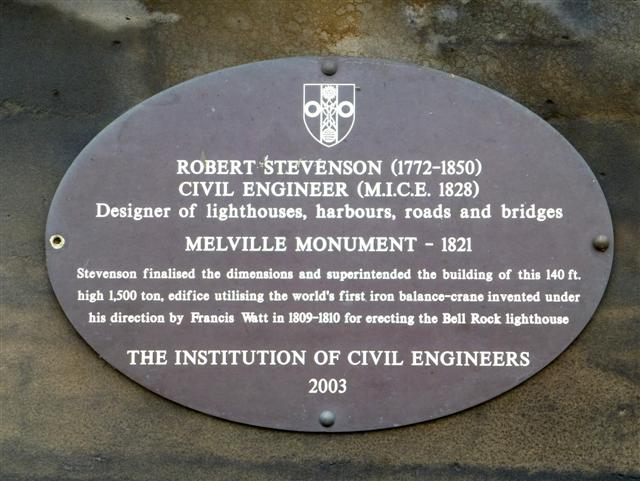
\includegraphics[width=1\linewidth]{img/stevenson_plaque.jpg}
    \caption{Close-up of plaque to finalising engineer of the Melville monument}
    \label{fig:stevenson_plaque}
\end{figure}
\begin{figure}
    \centering
    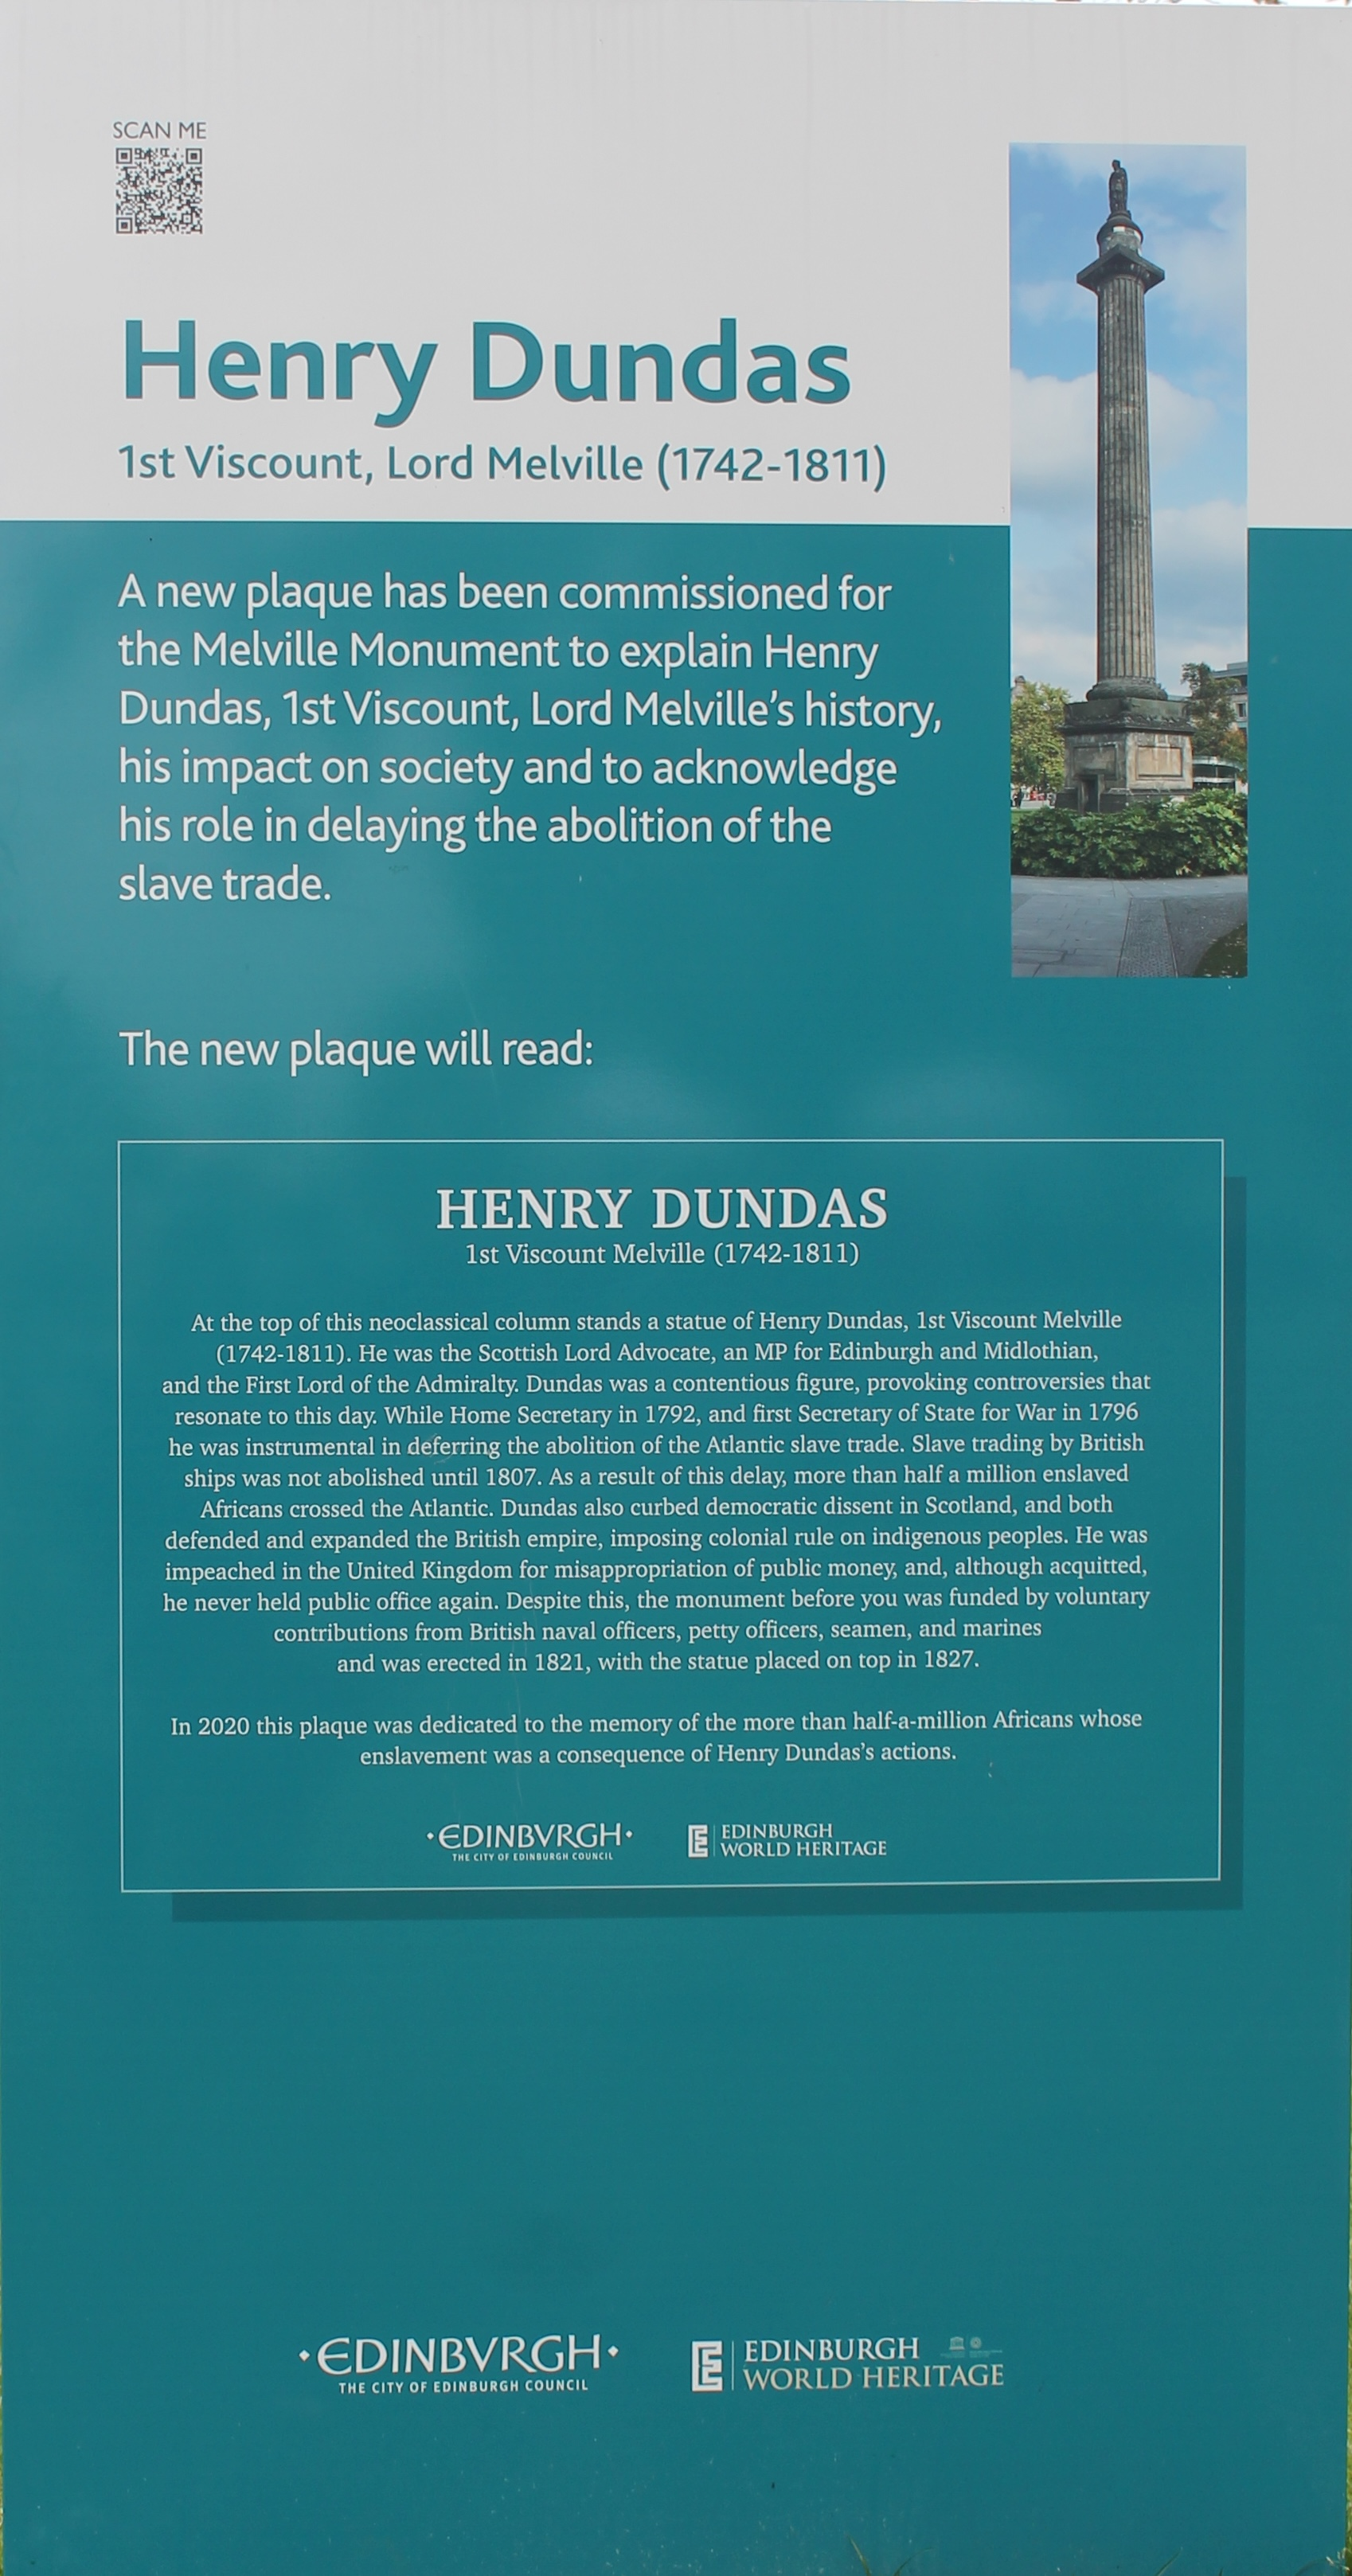
\includegraphics[width=0.75\linewidth]{img/melville_temp.jpg}
    \caption{Temporary Information Board}
    \label{fig:temp_info}
\end{figure}
\begin{figure}
    \centering
    \includegraphics[width=1\linewidth]{img/melville_dirt.jpeg}
    \caption{Monument as viewed from the path at St Andrews square}
    \label{fig:melville-dirt}
\end{figure}

\begin{figure}
    \centering
    \includegraphics[width=1\linewidth]{img/melville_dirt_plaque.jpeg}
    \caption{Base of Melville's Monument as viewed from the path through the square facing  west}
    \label{fig:melville-dirt-plaque}
\end{figure}

\begin{figure}
    \centering
    \includegraphics[width=1\linewidth]{img/temporary_info.jpeg}
    \caption{Temporary Information Board as viewed from the North-East Entrance to the square}
    \label{fig:temp-info-square}
\end{figure}

\begin{figure}
    \centering
    \includegraphics[width=1\linewidth]{img/paddington.jpg}
    \caption{Paddington Bear in front of Melville Monument}
    \label{fig:paddington}
\end{figure}

\begin{figure}
    \centering
    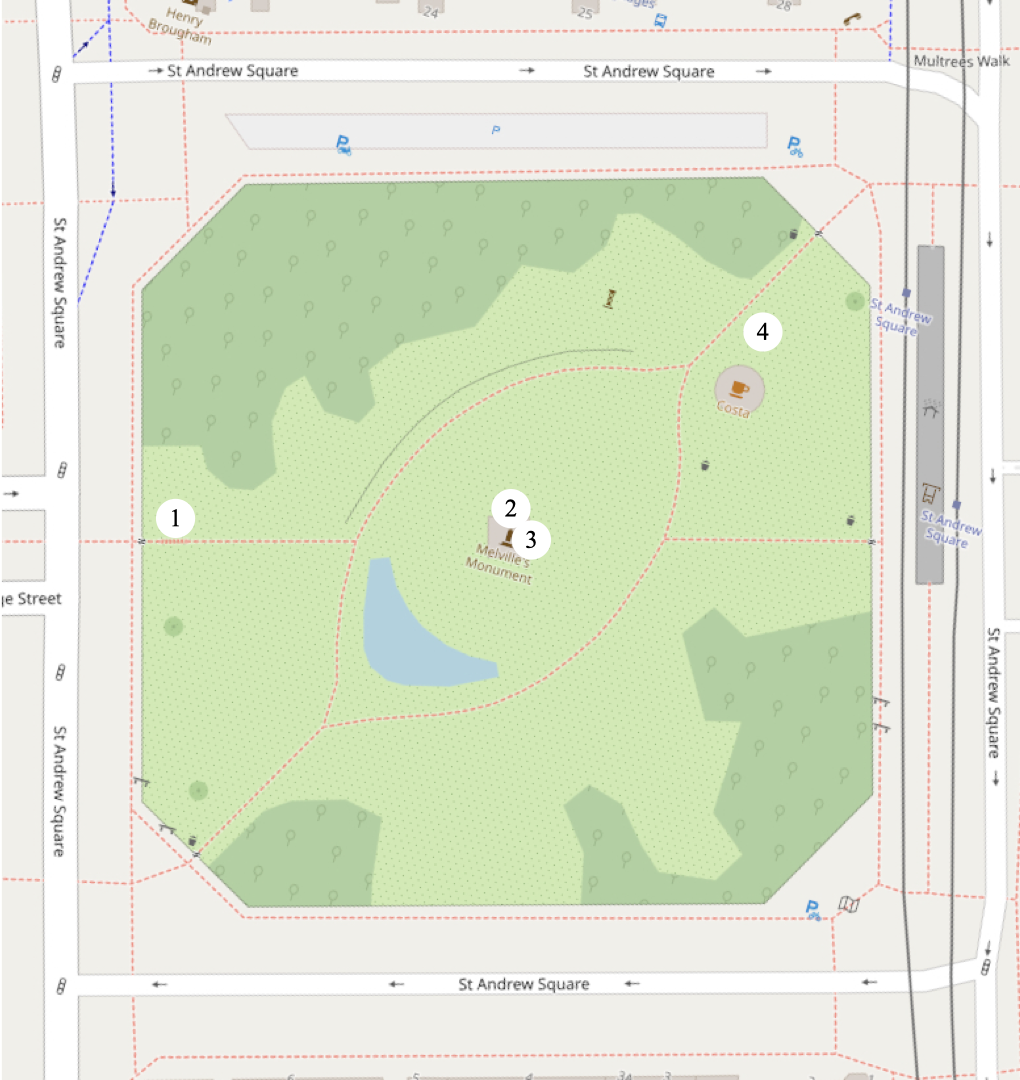
\includegraphics[width=1\linewidth]{img/map_numbered.png}
    \caption{Map of St Andrews Square (Source OpenStreetMaps.org), position of the plaques are \textbf{1.} Original \textbf{2}. Updated \textbf{3}. Stevenson \textbf{4.} Temporary}
    \label{fig:st_andrews_map}
\end{figure}

\begin{figure}
    \centering
    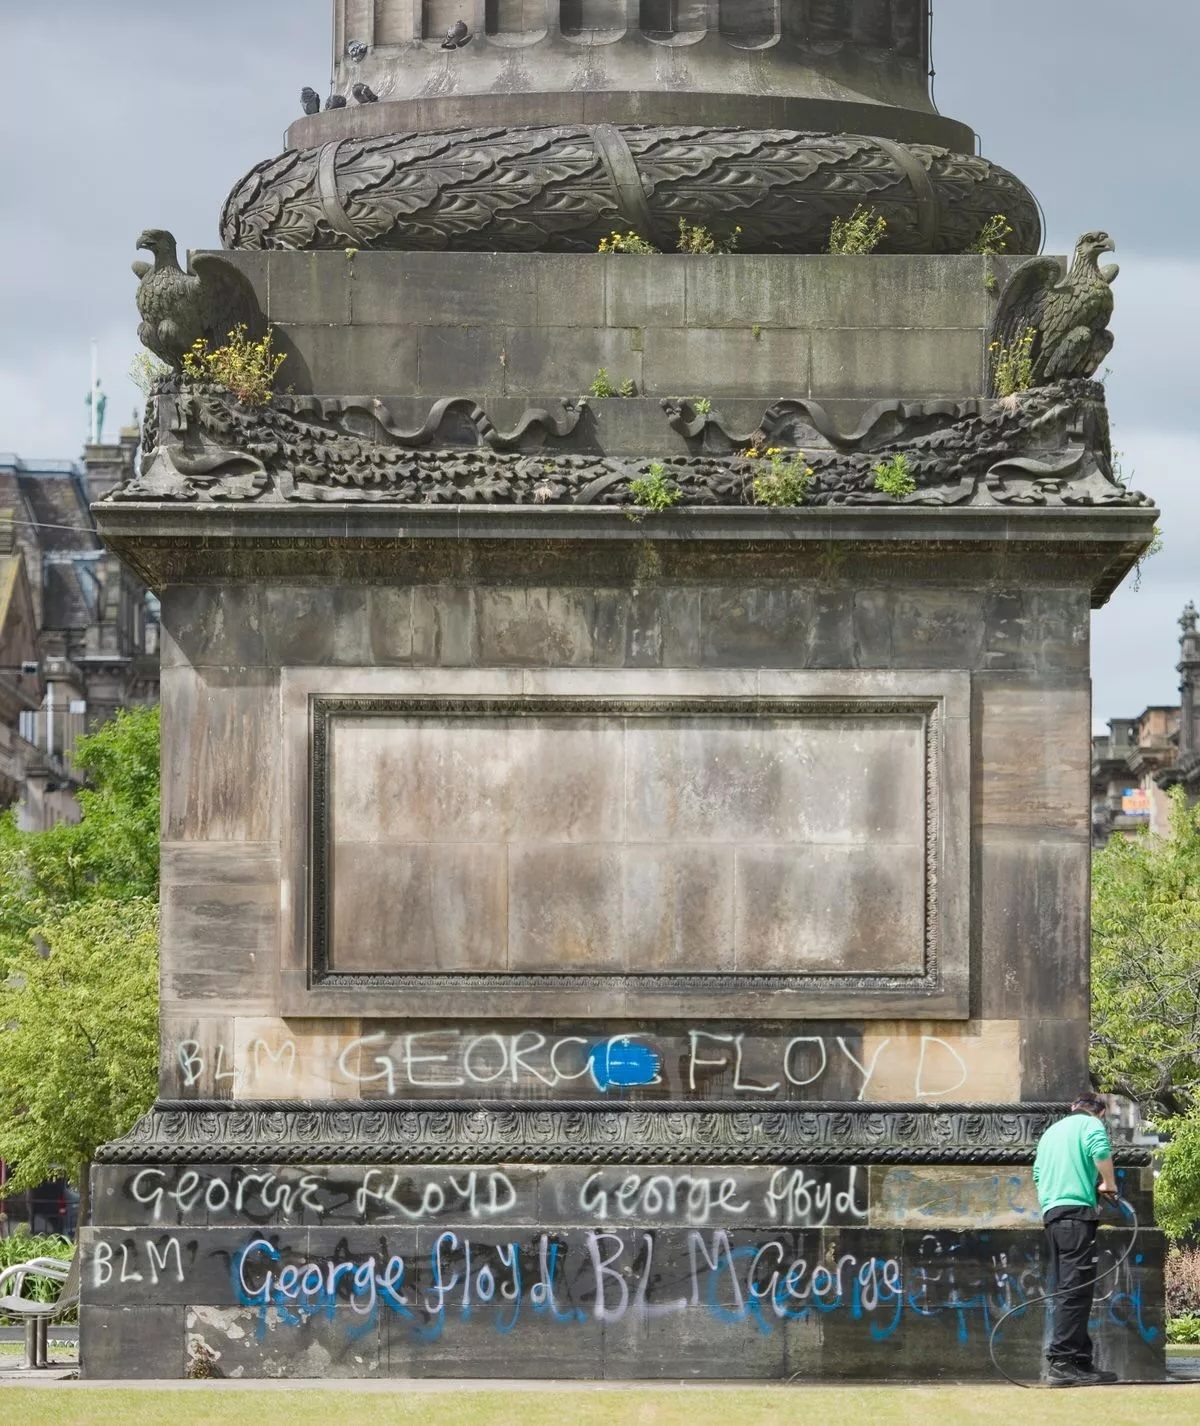
\includegraphics[width=1\linewidth]{img/melville_graffiti.jpg}
    \caption{Graffiti on Melville Monument: Source \cite{daily_2020}}
    \label{fig:dundas_graffiti}
\end{figure}
\begin{figure}
    \centering
    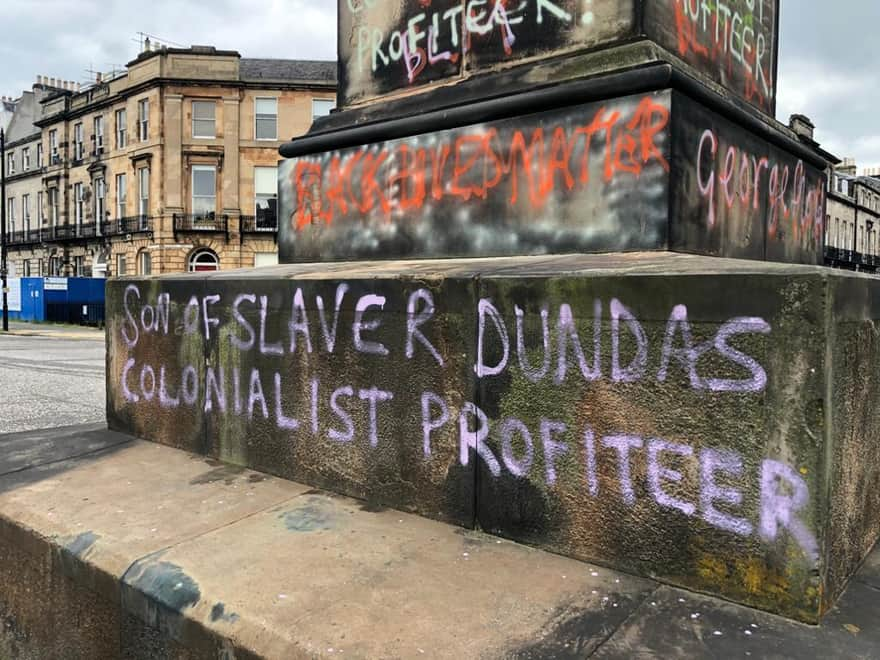
\includegraphics[width=1\linewidth]{img/robert_dundas_defaced.jpg}
    \caption{Graffiti on Robert Dundas Memorial. Source \cite{hay_2020_3}}
    \label{fig:robert_graffiti}
\end{figure}

\begin{figure}
    \centering
    \includegraphics[width=1\linewidth]{img/plaque-committee-2.png}
    \caption{The ``plaque committee''. Source Channel 4 News 
    \cite{c4n_2018}. From left to right: Bobby Dundas, Geoff Palmer, Unknown, Michael Fry, Adam Ramsay}
    \label{fig:plaque-committee}
\end{figure}
\end{appendices}

\end{document}
